\newpage
\part{Design}

    \graphicspath{{images/design/}}


    \section{Networks}
        
        \subsection{Network Frameworks}
        There were two main contenders for network frameworks to use - Pytorch and Tensorflow. Both of these frameworks are written for python and are widely used, so very well documented.

        In the end pytorch was chosen for its simplicity, versatility and speed of training \textbf{INCLUDE CITATION HERE}. The more high-level features of Tensorflow to do with deployment or distributed training were not needed. 


        \subsection{Data in/out}

        Each model should be able to work with 4 points of data at every time unit: open, high, low, close, or less. This is to fit the structure of incoming/real-world data provided by the AlphaVantage api (FX Intraday). 

        To train/test our agents, a dataset of open/high/low/close/volume from a six year period on the EURUSD market with 15 min intervals will be used. We will start tests using an 80/20 split of training data to test data, as this is a good balance between ensuring that the agent learns enough during training and accurately assessing the agent's ability. 

        Neural networks work better when inputs are normalised i.e. take on values between -1, and 1. To achieve this (or at least a proxy for this), raw input values were changed to 
        
        \begin{equation}
        (value - meanClosePriceOfWindow) \times 100
        \end{equation}

        The window is the time range for which the network is given inputs. Even for large windows, inputs to the network would very rarely exceed 1 or -1.

        For outputs the inital plan was to let the network choose from one of three options - the price at a timestep will be within the spread of, or greater/lower than the spread of the most recent timestep. The spread was chosen for this as broker fees are often in the form of spread \textbf{see **}- the price must "clear" the spread in order for a trade to return a profit and so seeing if a trade will go beyond the spread is useful. Each option would have a confidence level - the percentage chance the network attributes to that outcome.

        \subsection{Proposed Networks}

        We have two problems to consider with the how inputs to the network. Firstly we need the network to be able to see many previous time steps as this is what will likely allow it to predict prices correctly if anything. Secondly, for each time step, we have 4 data points - open, high, low, close.

        A variety of input arrangements were proposed for the networks.

        \begin{itemize}

            \item \textbf{Feed-forward Networks:} All the feed-forward networks below would have a 1D convolutional layer as the first input layer, convolving each of the four inputs for a timestep (open, high, low, close) and producing one output for the next layer

            \begin{itemize}
                    
                \item \textbf{Normal deep learning network:} The network would be made up of standard feed-forward connections in which every ouput in one layer would be an input to every node in the next layer. While straightforward to implement, this requires many neurons to train 

                \item \textbf{Casually dilated convolutions:} This technique was inspired by Deepmind's wavenet \cite{wavenet}. It has the advantage of being able to look back on many previous timesteps while having a relatively small number of neurons to train. The structure of the network has the shape of a binary tree, where each layer has half the neurons of the last and each neuron takes two inputs from the previous layer. This allows the network to have a large lookback period without requiring many neurons.
            
                \item \textbf{Exponetially increasing merged timesteps:} This setup is motivated by the assumption that the further back in the past the data is, the less relevant it is. For this, we will take current set of 15 min data (0 to -15), the set of data from -15 to -30, then -30 to -60, -60 to -120, -120 to -240 and so on (if needed). To merge timesteps, we take the open value of the timestep furthest back in the past for the window we are looking at, the close from the most recent, and the maximum high value and minimum low value throughout the range. 
            
            \end{itemize}

            \item \textbf{Recurrent Networks:} Recurrent networks are good at solving problems that have a sequential nature, such as time series problems. Because of this, they are very appropriate for the problem at hand, however they take longer to train \cite{wavenet}.
            
            \begin{itemize}

                \item \textbf{LSTMs}: LSTM (Long-Term Short Memory) networks are especially good at solving sequenced problems as each lstm unit in the network chooses to remember of forget certain values depending on how important the network deems the value to be.
                
            \end{itemize}

        \end{itemize}

        It was decided that a feed-forward network with "normal inputs" and a recurrent network should be tested before the other feed-forward networks as they would be more difficult to implement


        \subsection{Training Process}

            \subsubsection{First Network}
            The initial model was a normal deep learning network. N previous sets of OHLC data were fed to the network and 3 outputs were given, representing the probability the network gave to the price moving up, down and staying within the typical spread price.

            As discussed above, the first layer was a 1D convolution that created one output for each set of OHLC data. For the other hidden layers, a number of setups were tested, with usually a starting layer of 64 neurons. The output layer had three neurons with a softmax \footnote{A softmax is a function that normalises a number of values. This is often used to get probabilities from an output layer.} applied so the network outputs represented the probability the network assigned to the price moving up, down, or staying within the spread. The network was initially setup with the SGD optimiser, with a small learning rate of 0.01 as is customary for deep supervised learning.
            
            \begin{figure}[h]
                \centering
                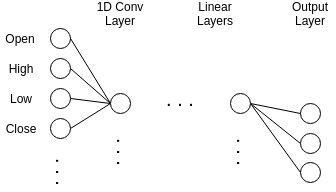
\includegraphics[width=0.8\textwidth]{Conv-Net.png}
                \caption{Network Diagram}
                \label{fig:first_net_diagram}
            \end{figure}

            As a preliminary test, it was decided the network should try to overfit \footnote{Overfitting is where a network learns the test data and corresponding outputs it is given instead of being able to generalise and learn which features of the inputs cause certain outputs, thus performing very badly on unseen data. This usually happens when the size of the test data is too small} on a small batch first. The network greatly struggled with this however. On every run the network would either converge on a solution that assigns equal probability to each outcome, or one that always assigns 100\% to the price increasing or decreasing.

            Eventually, using the “Adam” optimiser instead of SGD, the network managed to overfit on the small batch of 20.\footnote{In Fig.~\ref{fig:Overfit} the rows above show the output tensors from the network for the last few inputs. Below the expected outputs vs. the network ouput with the largest value (the network prediction)}

            \begin{figure}[h]
                \centering
                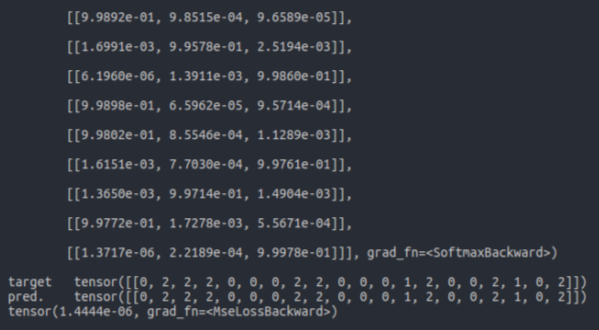
\includegraphics[width=0.8\textwidth]{overfit.png}
                \caption{Output from running the overfitting test.}
                \label{fig:Overfit}
            \end{figure}
            

            It was thought that the reason Adam worked was because the problem is quite complex and thus SGD (steepest gradient descent - which takes steps only in the direction of the steepest gradient) was less likely to have found the global minimum of the cost function, whereas Adam, which is stochastic, is better at “exploring” the landscape of the cost function and so more likely to find the global minimum.

            When attempting the actual training (using the entire training dataset), all runs gave unsatisfactory results. At best networks gave the correct prediction around 49\% of the time. Given that at the 15 minute interval the price moves up/down around 45\% of the time and stays within the spread the remaining 10\%, the network was not giving desirable predictions (the network was barely doing better than random guesses).

            The approach that was taken to this problem of mapping the inputs onto one of three discrete outputs was influenced by classic classification problems such as recognising images of handwritten digits in which there is a clear "correct" mapping between the inputs onto one output. However forex prices are stochastic - it is possible to determine with certainty given a set up of inputs what the "correct" output should be so it was thought that training a network using the three discrete outputs (price up, down, same) represented as a [1, 0, 0], was causing problems during optimisation.

            It was decided that a network with a different structure should be tested.


            \subsubsection{LSTM Network}
            It was decided that the next test should be an LSTM network that predicted the price itself. N individual sets of OHLC values would be fed one by one into the network with one LSTM layer and one single output neuron. The Adam optimiser was used with learning rates from 0.05-0.4.

            \begin{figure}[h]
                \centering
                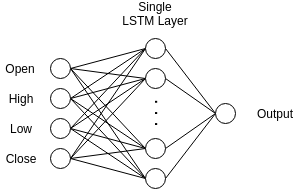
\includegraphics[width=0.8\textwidth]{LSTM-Net.png}
                \caption{Network Diagram}
                \label{fig:LSTM_Diagram}
            \end{figure}

            The network produced what were thought to be far more desirable results, with initial tests able to predict the price in 15 mins correctly within the spread (taken as 0.7 pips) roughly 60\% of the time . This was initially surprising as originally, it was initially thought that predicting the price itself was a more difficult problem than just predicting the discrete movement of the price.

            When graphing the prediction values against the actual prices at that timestep however, there was a concern that the networks were only achieving these results as it seemed to be just quoting the most recent close price for as the prediction for future timesteps.

            \begin{figure}[h]
                \centering
                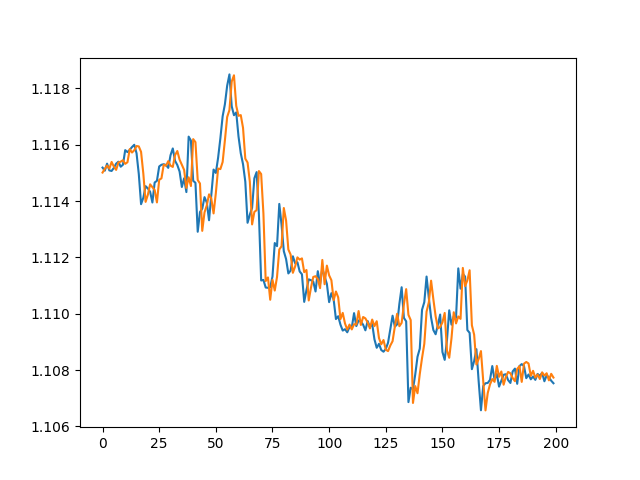
\includegraphics[width=0.8\textwidth]{30-40-15-2.png}
                \caption{Sample prices (blue) against the prediction (orange) made for the price at that timestep 30 minutes (2 timesteps) beforehand}
                \label{fig:30_predictions}
            \end{figure}

            In Fig.~\ref{fig:30_predictions}, the predictions series looks almost exactly the same as the actual price series, just displaced 2 timesteps. 

            There were a few ideas about why this might have been the case and how to improve on it.

            \begin{itemize}
                \item \textbf{Too few neurons} The network was not large enough and so couldn't learn the more complex behaviours required.
                
                \item \textbf{Window size was too large} Too much data was being fed to the network. With so many inputs it was difficult for the network to converge on a valid solution other than quoting the latest close price. Additionally, network outputs were given as movements from the mean of the window so the larger the window, the larger the window, the greater the variance of the mean in relation to the final close price, which could be affecting the validity of the predictions. 
                
                \item \textbf{Prediction time-scale too small given the data} The tests were first being done on 15 and 30 minute predictions. Given the data being fed to the network was in 15 minute intervals, it was thought that these predictions could have been too close in the future for the network to converge on effective solutions as the price would not have moved too far/any movements had too much associated noise. It was thought that over longer time-scales general trends would be able to be found and thus more effective predictions could be made.
            
            \end{itemize}
            

            It was found that adding more neurons could often result in a worse solution, likely because the network was too complex and the number of training iterations was too small to be able to properly explore the landscape of the fitness function. When decreasing the window size, it was found that the network could converge on smaller losses, and when doing tests on the predictions further in the future, returned values were thought to be better.

            \begin{figure}[h]
                \centering
                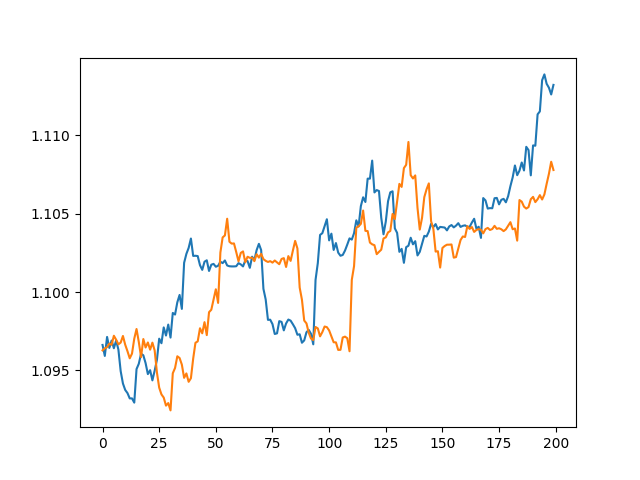
\includegraphics[width=0.8\textwidth]{240-50-30-1.png}
                \caption{Sample prices (blue) against the prediction (orange) made for that timestep 4 hours (16 timesteps) beforehand}
                \label{fig:240_predictions}
            \end{figure}

            In Fig.~\ref{fig:240_predictions} while it does seem that the network mostly seems to be quoting the most recent close price, at many points we can see that it is both over and undershooting peaks and troughs - showing that it is observing trends and making decisions based on data from more than just the last timestep.

            It was decided that this structure should be used in the final solution.


        \subsection{Measuring Success}

        Now it had been decided that a raw price prediction network would be used, the ability of a network was measured by two criteria - the mean squared error between the predictions and the target values, and the percentage of predictions made that fell within the high and low prices of the relevant timestep.

        As discussed above, it seemed as though the network could have been just quoting the most recent close price as the prediction. To test this - ensure the network was making "valid" predictions, a baseline was created by finding the MSE and percentage accuracy of a solution quotes the most recent close price as the prediction for a future timestep. 

        It was decided that that networks would be evaluated against the baseline's MSE and percentage accuracy.


        \subsection{Saving/Loading Networks}
        To be able to use the models, the trained parameters need to be saved. This quite straightforward to do in pytorch luckily. The current parameters of a network can be written to a file in a custom pytorch format to save a trained network. To load in a network from this file, when an instance of the original network class is initialised, the file can be parsed to the network. 
        
        Thus for each network being used, both the trained parameters and data about the network structure needs to be stored.


    \section{User Interface}

        The site should have three pages - the "main" page, which displays the predictions and accuracies, an "API" page where a user can get enter an API key as well as see a sample request/sample returned datafile and and "About" page in which the functionality of the site is explained.

        When a user enters a valid email that is not currently in the database, they will be redirected to a separate page that displays their API key and some messages about good usage.

        Using the above, the structure of pages of the site is shown in Fig.~\ref{fig:site_layout}

        \begin{figure}[h]
            \centering
            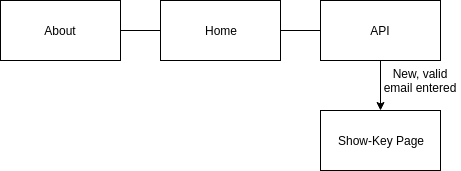
\includegraphics[width=0.8\textwidth]{Site Layout.png}
            \caption{Diagram of the layout of the site}
            \label{fig:site_layout}
        \end{figure}

        On all there should be a clear navigation bar which allows the user to easily move between pages of the site. There should be some indication of the current page the user is on.

        \subsection{Main Page}
        The predictions should be shown in a concise way graphically so that users viewing predictions via the webpage can more easily interpret the data. All data should be shown on one page.
        
        It was thought that previous market data, predictions as well as some measure of the precision of the predictions such as standard deviation of error should be displayed on one graph. If possible users should be able to choose how much historic data/how many predictions are being displayed at one time using sliders. The idea behind this is that it would help users interpret the data better - when all relevant data is displayed on the page the graph it was thought that the graph might appear to be too "noisy". On the same page, there should be a chart displaying the recent accuracy of predictions (how often the network correctly predicts the price within the actual high and low of the timestep). 

        On the page the current UTC time and the time of the data being shown should be displayed.

        As the market is closed on weekends/AlphaVantage doesn't update data over the weekend, there should be a message on the home page to tell users that prices aren't being updated if it is between Friday 10pm and Sunday 10pm.

        A mock-up of the main page is shown in Fig.~\ref{fig:main_page_mock} 

        \begin{figure}[h]
            \centering
            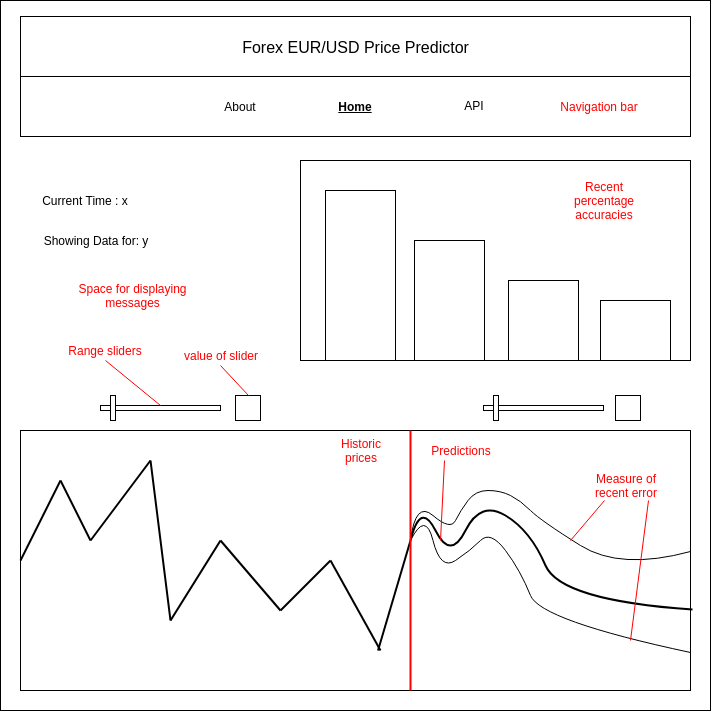
\includegraphics[width=0.95\textwidth]{Main page mockup.png}
            \caption{Mock-up of the main page}
            \label{fig:main_page_mock}
        \end{figure}


    \section{API}
        
        \subsection{Data Returned}
        When an API call is made, the server will check if the API key used is valid (is in the list of API keys being used). If it is, then data will be returned, else an error message will be returned.

        Data returned should be in JSON format and include all data that is shown on the webpage in numerical form. JSON was chosen as it is relatively compact, well supported and also allows for more logical representation and ordering of data with the use of hierarchy. 

        A request should not be served if requests from the user are being made too frequently.
    

        \subsection{Signing Up}
        On the webpage, there should be a text field where a user can enter there email to get an API key. If the email is valid, a random API key will be generated and sent to the user. If the email is invalid an error message should appear. If the email has already been used to sign up, the API key should be shown.

        \subsection{Email Hashing}
        It is thought that the users would never need to be directly contacted and thus the user emails should never be stored or sent in plaintext to ensure user privacy. Were emails sent in plaintext, a "man in the middle" would be able to see the email.

        To ensure this, when a user signs up for the service their email should be hashed on the client side with a random salt before being sent to the server. The user will then be shown their API key on the webpage. The hash algorithm used should not be too complex so as to ensure that there's not too much time between a user entering their email and receiving a response. The size of the hashed value should be large enough that there is a negligible chance of collisions occurring given the number of users who are expected to use service.

        When the hashed email is sent the server on signup, the table of current users will be queried to find if the API key is already being used. If it is, then the user is returned their API key with an existing  
    

        
    \section{Back-End}

        It was decided that flask should be used as the web framework. Much like pytorch, it is lightweight, versatile, easy to use and the advantages that other similar frameworks such as Django provide were not thought to be necessary for the end product.

        \subsection{Dataflow}
        There should only be one copy of historic data and predictions to ensure data is consistent in all places and updating these is easier. Because of this, the same datafile that can be accessed via the API should be used as the source of data for the webpage. This means that all data would be kept in a JSON format as prices retrieved from AlphaVantage are in JSON format and it was decided that predictions returned from the site API would also be JSON.
            
            \subsubsection{Updating data}
            Every 15 minutes, the server should check for new data from AlphaVantage. Data from the API does not update every 15 minutes on the dot however, so the server should keep making API calls until the time of the data changes. AlphaVantage stops fulfilling requests if they exceed more than 5 requests a minute or more than 500 requests a day. Given that new data for each 15 minute timestep seemed to come roughly 5 minutes late, a 45 second delay between requests was thought to be appropriate.

            Once new data has come in from AlphaVantage, it should be processed and fed to all the models to produce a new set of predictions as well as compared with previous predictions to determine the recent performance of the networks

            Fig.~\ref{fig:updateDataFlow} shows data flow diagram for the updating process.

            \begin{figure}[h]
                \centering
                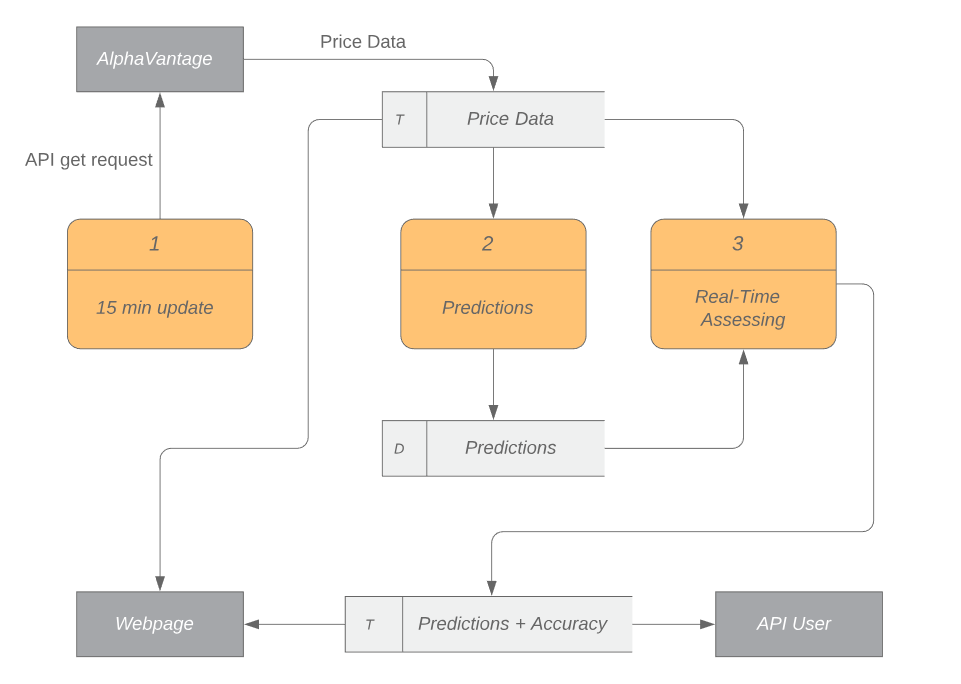
\includegraphics[width=0.8\textwidth]{updateDataFlow.png}
                \caption{Data flow diagram for the update process}
                \label{fig:updateDataFlow}
            \end{figure}
            

        Note above that "Price Data" (data from AlphaVantage) and "Predictions + Accuracy" (data sent by API) are represented as temporary data stores while "Predictions" are a permanent data store. For each new set of 15 minute price data coming in, the JSON files for the price data and the predictions + the accuracy are overwritten with the new values for the current timestep. It was thought that price data would not need to be stored as it will likely be readily available elsewhere if needed. Thus in only storing all predictions, data for predictions is not duplicatied, reducing data store and by using historic price data any new desired statistics about prediction accuracy can still be calculated.
        
        \subsection{Database}
        To allow for the API functionality outlined, each user's email hash and the corresponding needed to be stored as well as the timestamp of the most recent API request to ensure the user is not making requests too frequently. It was thought that keeping a record of all requests could be beneficial as it would allow user metrics such as total and individual activity to be calculated, allowing for an insight into user behaviour. Storing this data would mean that the timestamp of each user's last request need not be stored as it could be found by querying the list of all requests.

        The predictions made at each timestep also needed to be stored to allow for real-time assessing of the networks' ability.
        
        Thus it was decided that the tables required would be as follows
        \begin{itemize}

            \item \textbf{User:} Stores Email hash, API key, Date of signing up. 

            \item \textbf{Request:} Stores the time of the request, the user ID and if each request was served.
            
            \item \textbf{Predictions:} Stores the timestep that the predictions were made for (i.e. some multiple of 15 minutes <= the time at which predictions were made instead of the time at which the predictions were made themselves) and all the price predictions.
            
        \end{itemize}
        
            \subsubsection{Normalisation}
            The database should be normalised in order to make querying and managing tables easier. It was decided that normalising up to third normal form would be appropriate as forms beyond this are rarely used in practise \textit{add citation https://mariadb.com/kb/en/library/database-normalization-5th-normal-form-and-beyond/}. With the proposed structure, the database will be designed so that it passes all the forms below.

            \begin{itemize}

                \item \textbf{1st Normal Form:} Values in each field must be atomic i.e. each first stores one value. The only consideration for this is the predictions table - each prediction should be in their own column
                
                \item \textbf{2nd Normal Form:} Every non-key attribute of a table with a composite key, should depend on the whole key. The request field is the only table that is relevant to this as it has a relation to the user table. To help avoid this, the request table will just user a standard numeric primary key.
                
                \item \textbf{3rd Normal Form:} Fields have no dependencies on other non-key fields. The database is quite small overall - there are no problems with non-key dependencies. 
            
            \end{itemize}

            \subsubsection{Final Database Structure}
            Following the discussion above, it was decided the final database structure should be as shown in Fig.~\ref{slidersdb_table}. It satisfies 3rd normal form.

            \begin{figure}[h]
                \centering
                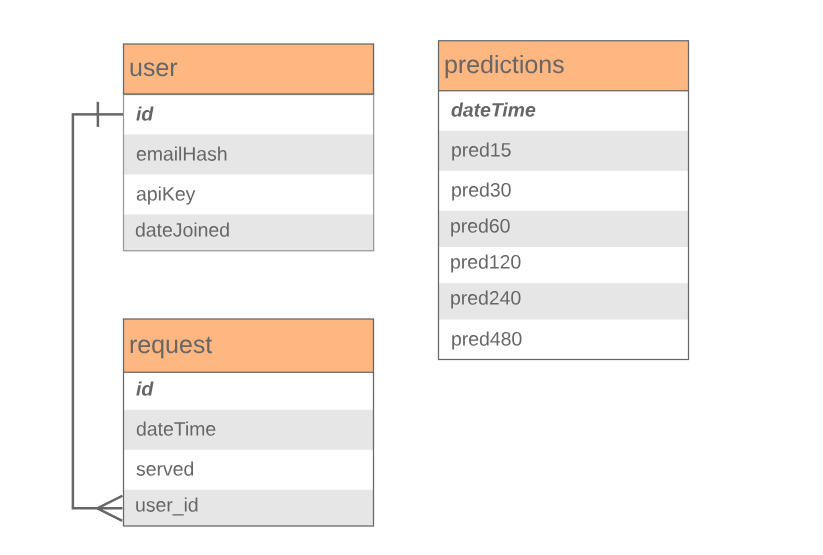
\includegraphics[width=0.8\textwidth]{tables.png}
                \caption{Entity relationship diagram}
                \label{fig:db_table}
            \end{figure}
            
            The user table is defined as follows:

            \begin{tabular}{|p{2cm}|p{2cm}|p{7cm}|}
                \hline
                \multicolumn{3}{|c|}{user} \\
                \hline
                Field & Type & Description \\
                \hline
                id & INT & primary key - uniquely defines each user \\
                emailHash & VARCHAR (32) & hashed hex value of user's email+salt \\
                apiKey & VARCHAR (16) & random alphanumeric API key used for requests \\
                dateJoined & DATETIME & date that the user signed up \\
                \hline 
            \end{tabular} 

            The apiRequest table is defined as follows: An integer is being used as a logical boolean as SQLite does not have a boolean type.
            
            \begin{tabular}{|p{2cm}|p{2cm}|p{7cm}|}
                \hline
                \multicolumn{3}{|c|}{apiRequest} \\
                \hline
                Field & Type & Description \\
                \hline
                id & INT & primary key - uniquely defines each request \\
                dateTime & DATETIME & the datetime that the request was made \\
                served & INT (logical BOOL) & whether or not the request was served (1 is yes, 0 if no) \\
                user\_id & INT & foreign key to the user table \\
                \hline
            \end{tabular}
            
            The prediction table is defined as follows:

            \begin{tabular}{|p{2cm}|p{2cm}|p{7cm}|}
                \hline
                \multicolumn{3}{|c|}{prediction} \\
                \hline
                Field & Type & Description \\
                \hline
                dateTime & DATETIME & primary key - the time at which a prediction is made is unique to each set of predictions\\
                pred15 & FLOAT & the predicted price for 15 mins in the future \\
                pred30 & FLOAT & the predicted price for 30 mins in the future \\
                pred60 & FLOAT & the predicted price for 60 mins in the future \\
                pred120 & FLOAT & the predicted price for 120 mins in the future \\
                pred240 & FLOAT & the predicted price for 240 mins in the future \\
                pred480 & FLOAT & the predicted price for 480 mins in the future \\
                \hline
            \end{tabular}
            
            